\documentclass[dvisvgm]{standalone}
\usepackage{tikz}

\usetikzlibrary {arrows.meta,automata,positioning,shapes.geometric}
\begin{document}
    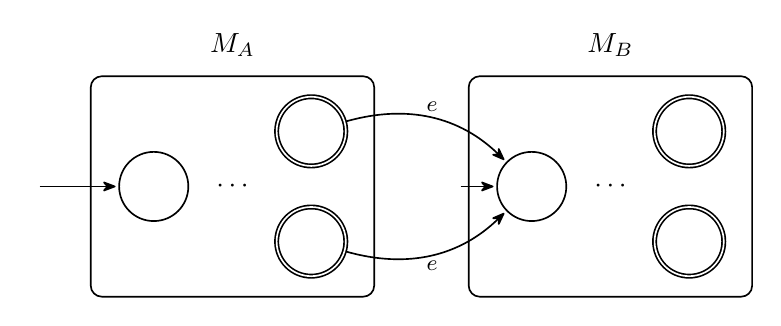
\begin{tikzpicture}[->,>={Stealth[round]},shorten >=1pt,%
        auto,node distance=2cm,on grid,semithick,
        inner sep=2pt,bend angle=30,initial text=]
        \node[initial,initial distance=1cm,state]       (q_0)   {};
        \node[state,accepting]          at (2,0.7)      (q_1)   {};
        \node[state,accepting]          at (2,-0.7)     (q_2)   {};
        \node                           at (1,0)        (dots)  {$\cdots$};
        \node                           at (1,1.8)              {$M_A$};
        \draw[rounded corners] (-0.8,-1.4) rectangle (2.8,1.4);
        
        \node[initial,state]            at (4.8, 0)     (p_0)   {};
        \node[state,accepting]          at (6.8,0.7)    (p_1)   {};
        \node[state,accepting]          at (6.8,-0.7)   (p_2)   {};
        \node                           at (5.8,0)      (dots)  {$\cdots$};
        \node                           at (5.8,1.8)            {$M_B$};
        \draw[rounded corners] (4,-1.4) rectangle (7.6,1.4);
        
        \path [every node/.style={font=\footnotesize}]
        (q_1)   edge [bend left]        node [above] {$e$} (p_0)
        (q_2)   edge [bend right]       node [below] {$e$} (p_0);
    \end{tikzpicture}
\end{document}